\chapter*{Métodos Estruturais para teste em nível sistêmico}
\addcontentsline{toc}{chapter}{Métodos Estruturais para teste à nível sistêmico}
\section{As bases do teste estrutural}

Mesmo em circuitos simples é impossível realizar uma verificação completa de sua funcionalidade, já que esta tarefa exigiria uma abrangência de entradas e estados que cresce exponencialmente. O problema é ainda mais difícil se circuitos analógicos ou de sinais mistos forem inclusos. Segundo Jutman (2014), um modelo estrutural de um sistema ajuda a diminuir significativamente a sua complexidade. O teste estrutural é composta pelos seguintes elementos:

\begin{itemize}
    \item Um modelo da estrutura do circuito (normalmente em nível lógico);
    \item Um modelo de falhas estruturais como faltas de transição de estados, atrasos, prisão de estado. Um exemplo genérico de modelo de falhas é o da prisão de estado condicional, que permite descrever praticamente todos os comportamentos de falta realísticos;
    \item Mudanças na estrutura do circuito pela adição de circuitos de \textit{design-for-test}, que podem introduzir modos de teste durante a operação;
    \item Padrões de teste estrutural, que detectam uma certa percentagem de faltas, isto é, alcançam a cobertura de faltas exigida.
\end{itemize}

Com estas modificações e acréscimos, o tempo e volume de dados de teste já não incrementam exponencialmente com o tamanho do circuito, mas linearmente (Jutman et al., 2014). Entretanto, nem todas as falhas podem ser cobertas pelo teste estrutural, pois as modelagens do circuito e das falhas não conseguem ser suficientemente precisas e o próprio modo de testes pode esconder falhas. Por esta razão, durante a manufatura são aplicadas estratégias tanto estruturais quanto funcionais \citep{zeng2004, maxwell2000comparing}, que serão vistas na próxima sessão.

\section{Reuso de esquemas de teste estrutural de semicondutores}

Como visto na tabela \ref{tab:boundaryscanfamily}, existem diversos padrões de \textit{design-for-test}; Alguns destes são usados no teste de semicondutores, outros paras placas, outros também para ambos. Atualmente, a maioria dos integrados contém estruturas proprietárias internas como caminhos múltiplos para sondagem interna, circuitos para compressão de dados e compactação dos resultados de teste, além de hardware para BIST autônomos até mesmo para lógica randômica como esquemas STUMPS\footnote{Arquitetura STUMPS (\textbf{S}elf \textbf{T}esting \textbf{U}sing an \textbf{M}ISR and a \textbf{P}SR\textbf{S}G: Conforme explicado em \citet{larsson2006introduction} a arquitetura STUMPS consiste no uso de MISR com PSRSG para a geração de vetores de teste e assinaturas}\citep{bardell1987built, jutman2014high}. % self testing using an MISR and a Parallel shift register sequence generator
% explica o que é stumps: Introduction to advanced system-on-chip test design and optimization Larsson, Erik
%https://books.google.com.br/books?id=lthW10jo2mUC&pg=PA44&lpg=PA44&dq=stumps+architecture&source=bl&ots=bT92RqJ_kB&sig=Yqi4k2Tg-eOo9-cxJn-HfT2DdJE&hl=en&sa=X&sqi=2&ved=0ahUKEwiNo93gzdLMAhVDlZAKHe70Ca8Q6AEILzAE#v=onepage&q=stumps%20architecture&f=false
% sobre stumps http://chips.ece.iisc.ernet.in/images/d/d2/1106.pdf
% sobre misr http://link.springer.com/article/10.1007%2FBF00153858
% http://www.cs.utah.edu/~rfonnesb/BIST.pdf
% http://www.eng.auburn.edu/~strouce/class/elec6970/bist10.pdf

Para o engenheiro de teste, parece natural reutilizar estas estruturas internas de teste de integrado também para o teste sistêmico da placa \citep{vo2006design, qian2009logic}. Mesmo assim, esta estratégia impõe desafios e criam potenciais problemas no que concerne à maneira de se trabalhar, proteção e segurança do sistema, especialmente considerando o reuso em diagnóstico em campo, que introduzem questões que serão discutidas a seguir.

\subsection{Acesso}

Mesmo que um sistema integrado possua circuitos de sondagem internos, os dados de teste precisam de alguma maneira serem entregues externamente. Embora esta seja a prática padrão realizada por equipamentos de teste automatizado (ATE) durante a manufatura, dentro de um sistema complexo, como um FPGA, isto precisa ser realizado por controladores especializados. Para estes casos, a já mencionada instrumentação centralizada por FPGA é uma maneira atrativa de implementar controladores de teste flexíveis (Jutman et al., 2014).

Outra questão que surge é a ausência de um meio adequado para os dados de teste serem transferidos -- como um barramento JTAG -- e, como uma forma de adaptação, os barramentos de comunicação existentes precisam ser reutilizados (Jutman et al., 2014). A figura \ref{fig:tamreuse} mostra um exemplo nos quais barramentos SPI e JTAG compartilham o mesmo meio de acesso para o transporte de dados de teste \citep{cook2012reuse}

\begin{figure}
\centering
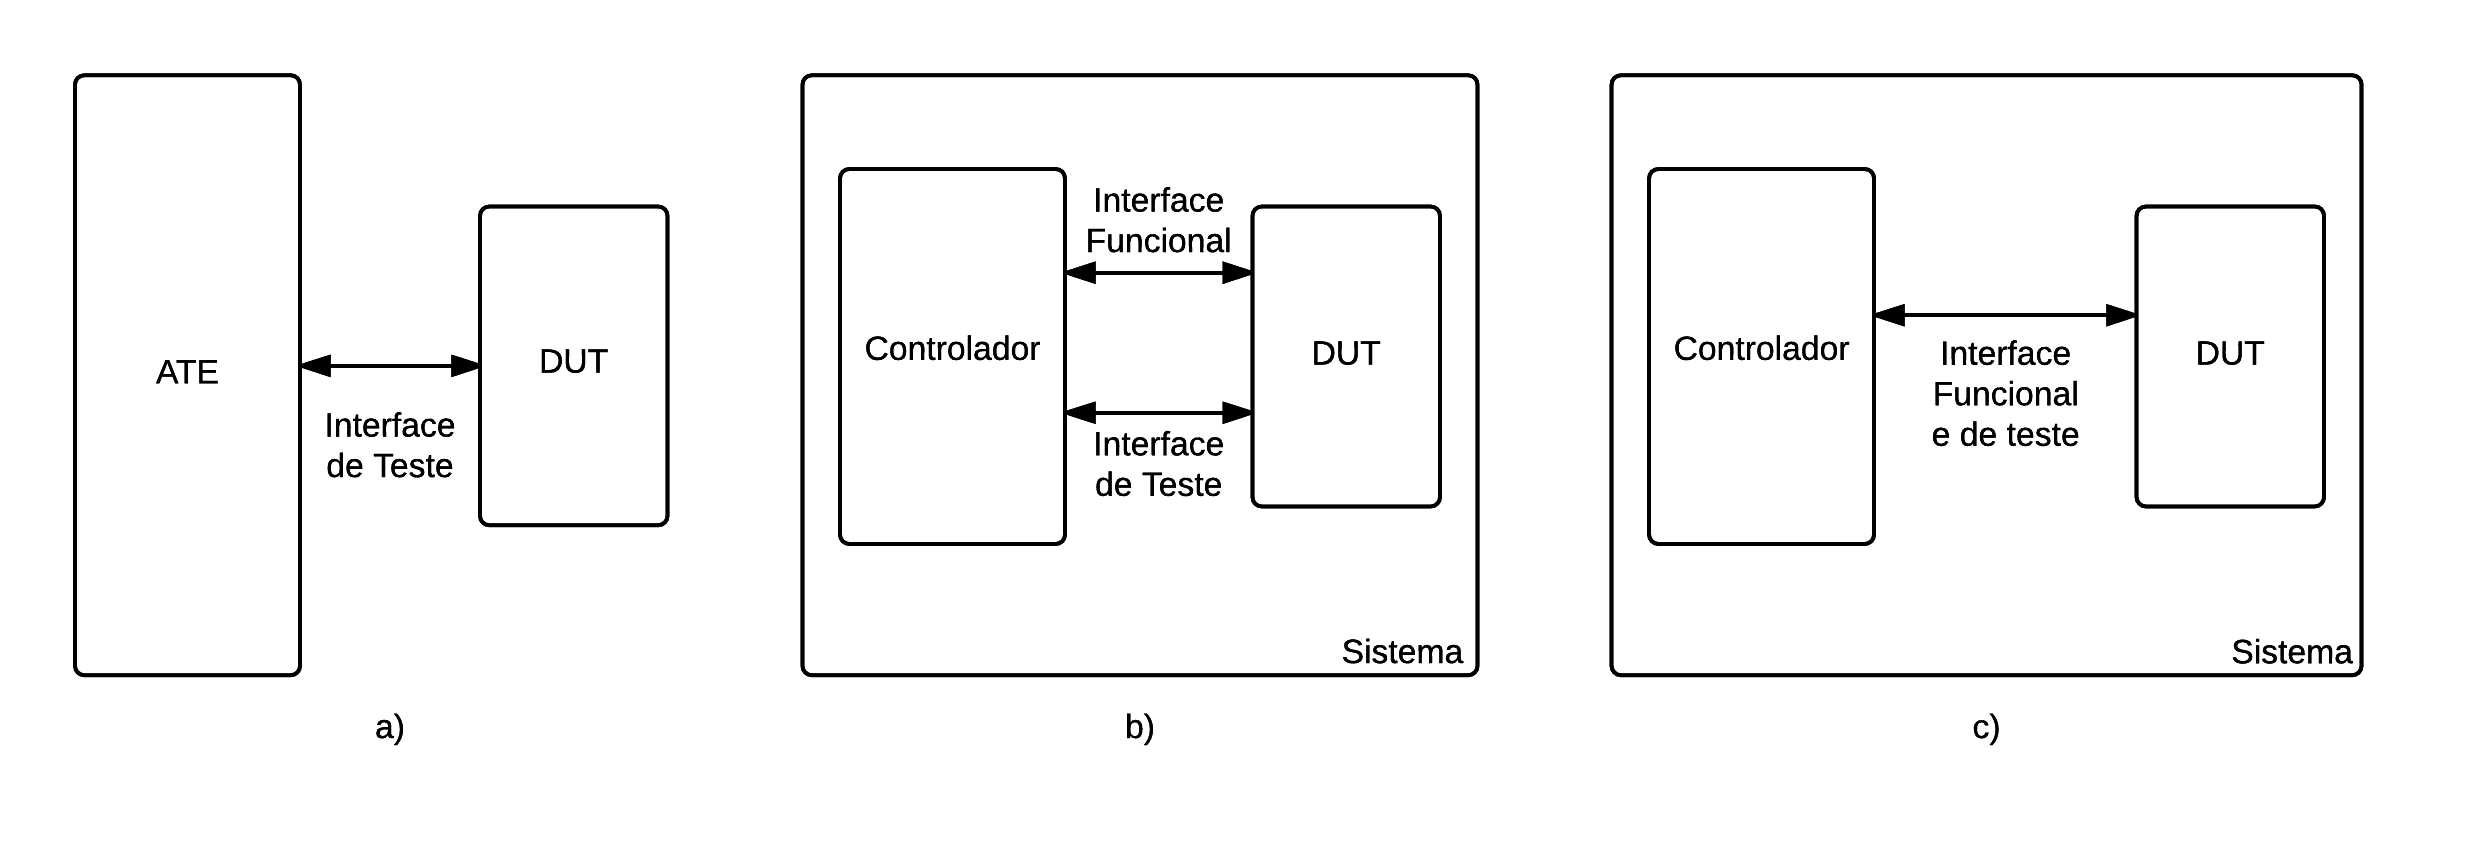
\includegraphics[width=1\linewidth]{tamreuse}
\caption{Reuso dos meios de acesso a teste. Retirado de Jutman (2014)}
\label{fig:tamreuse}
\end{figure}

\subsection{Dependência, proteção e segurança}
%rever toda essa parte pq n fez sentido
Segundo Jutman (2014), a abertura da infraestrutura de teste e diagnóstico vem também com um certo risco. É necessário garantir que esta infraestrutura não interfira na lógica do sistema e o acesso precisa ser restrito. Medidas de segurança precisam ser tomadas para garantir o acesso autorizado\citep{baranowski2013securing}.
A figura \ref{fig:mr} mostra diversas opções de restrição de acesso às RSNs.
\begin{figure}
    \centering
    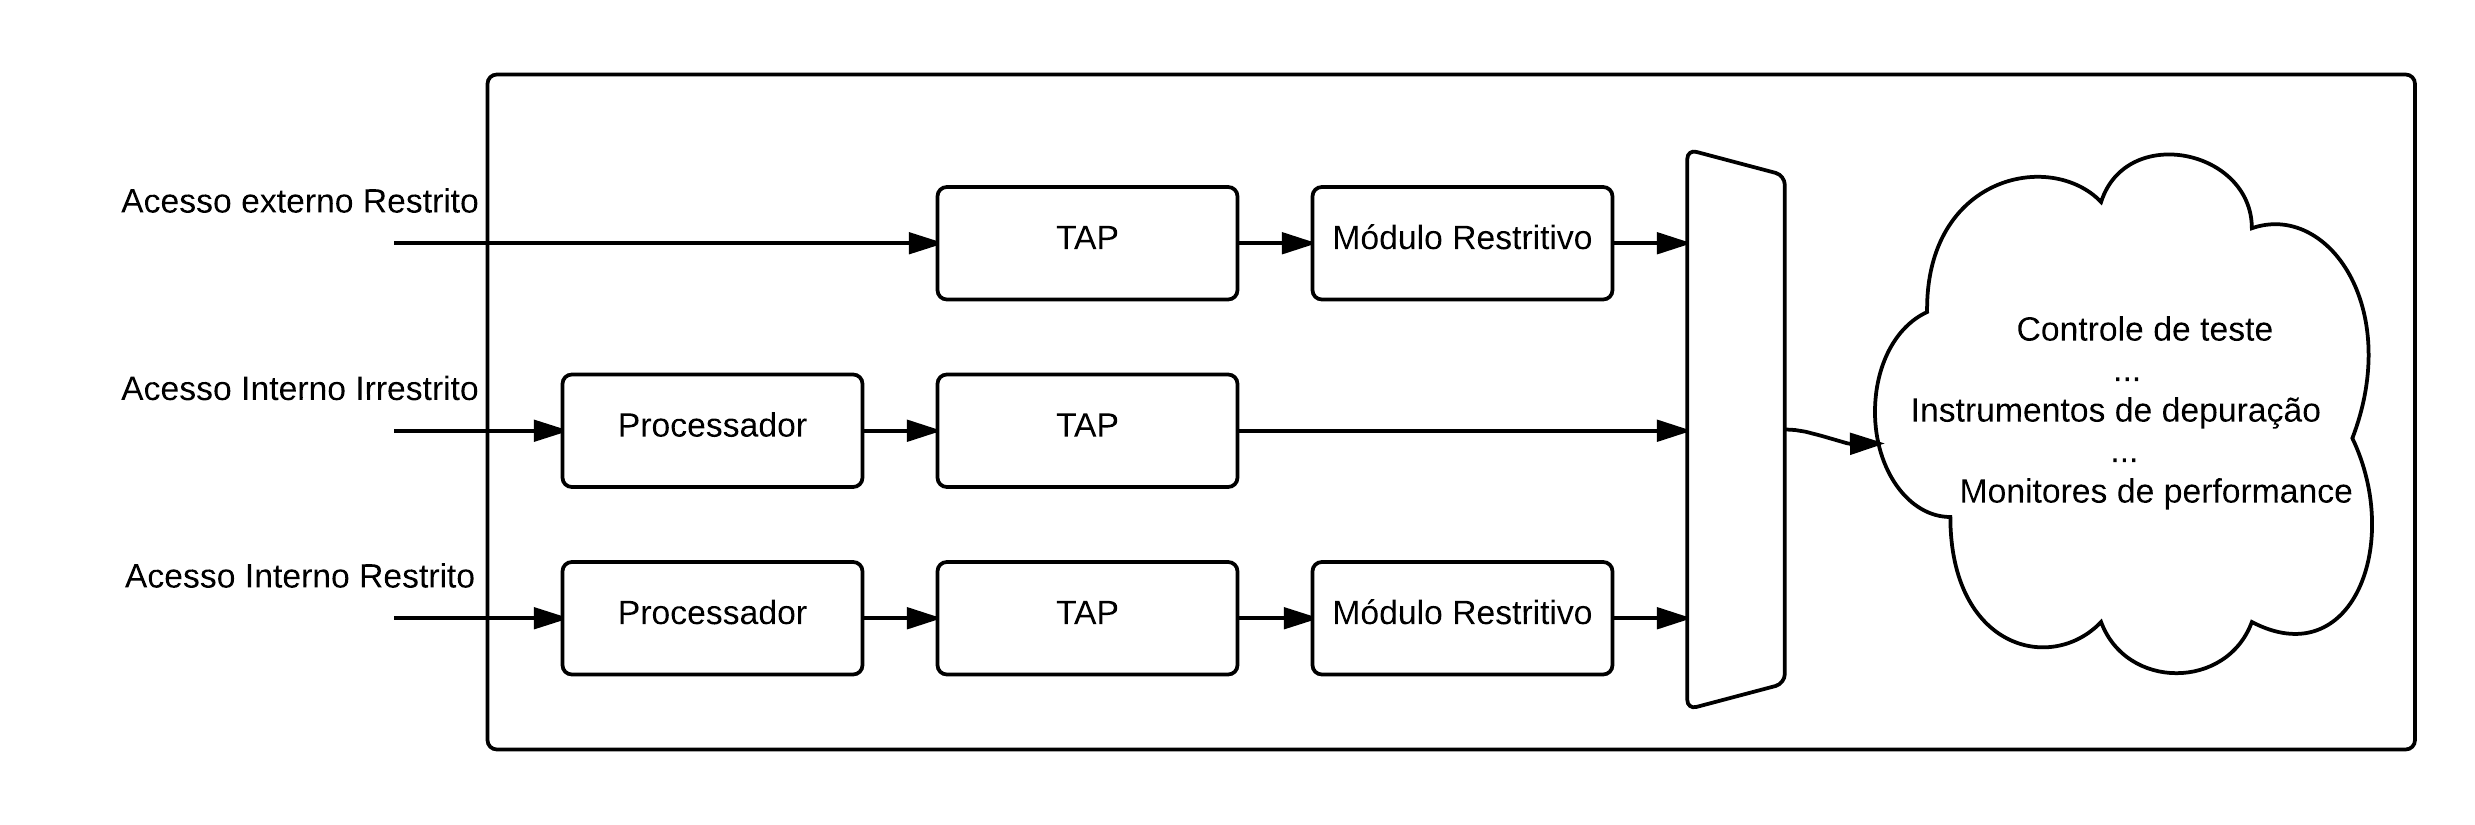
\includegraphics[width=1\linewidth]{mr}
    \caption{Restringindo acesso à infra de testes (Jutman et al., 2014)}
        \label{fig:mr}
\end{figure}
Jutman (2014) também apresenta como solução a introdução de um módulo restritivo (MR), que garante acesso para certas funcionalidades e estruturas de teste. Frequentemente, níveis diferentes de privilégios devem ser concedidos dependendo de autorização. Para a validação do sistema, análise de falhas de manufatura ou uma inspeção detalhada de retornos de campo, o acesso absoluto pode ser concedido. Numa oficina durante a manutenção, o acesso pode ser limitado para somente a coleta dos dados necessários para o reparo do sistema, e, para o usuário, pode-se somente permitir a coleta de checagens \textit{OK / Não OK}.

\subsection{Arquitetura \textit{on-chip} para diagnóstico embutido}
% a good reference for this http://eesemi.com/bist.htm
%https://en.wikipedia.org/wiki/Design_for_testing
%https://en.wikipedia.org/wiki/Automatic_test_pattern_generation
%

Como já mencionado, o auto diagnóstico embutido (BISD) concede o poder de pesquisa de faltas e defeitos sob às mesmas condições ambientais nas quais apareceram em campo sem que para isto seja necessário abrir ou obstruir o sistema. Entretanto, os esquemas BISD desenvolvidos para o teste durante a fabricação talvez não sirvam para o teste em campo, considerando as divisões do processo produtivo comparado ao contexto de operação em campo (Jutman et al., 2014). Se uma falta foi detectada durante a fase de autoteste, outras etapas adicionais são executadas para obter um diagnóstico intermediário e melhor localização da falta. \citep{cheng2007signature, wohl2002effective}\\

No caso de ASICS ou FPGAs, pode-se estender a arquitura STUMPS pela separação de três memórias: uma memória para os vetores de teste, outra memória de armazenamento de respostas para sinais intermediários, e uma memória de falha que armazena algumas assinaturas de falhas intermediárias, uma única etapa de teste é suficiente (ver figura \ref{fig:singlepass}).
\begin{figure}
    \centering
    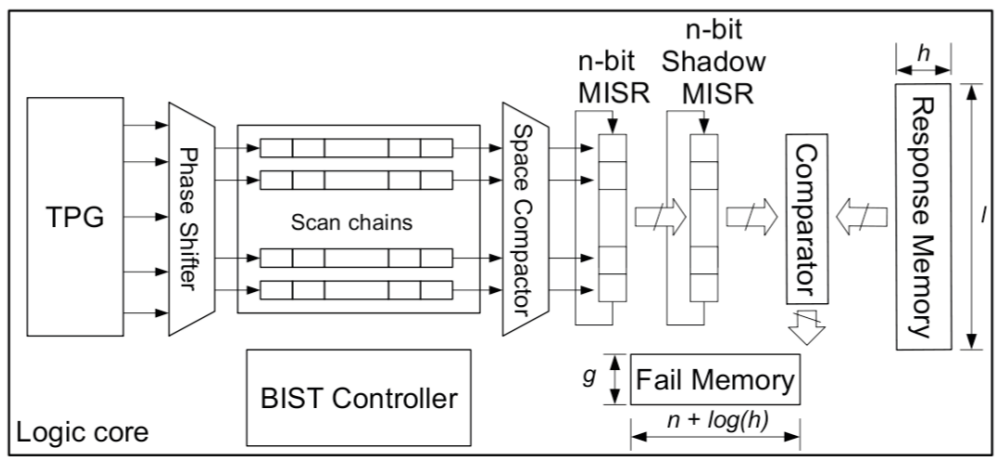
\includegraphics[width=1\linewidth]{bist}
    \caption{Esquema para um auto-diagnóstico embutido de passagem única (Jutman et al., 2014)}
    \label{fig:singlepass}
\end{figure}
O registrador MISR (Multiple Input Signature Register) coleta \textit{h} assinaturas intermediárias; cada uma delas é passada por um MISR "sombra" que roda alguns ciclos adicionais com a função de distribuir os últimos bits capturados uniformemente. As assinaturas corretas são armazenadas na memória de resposta e comparadas com as que foram capturadas. Em caso de diferenças, até no máximo \textit{g} assinaturas de falha, incluindo seus índices, são armazenadas na memória de falha. Assim, serão conhecidas até \textit{g} assinaturas de falha, e que as assinaturas entre elas estavam corretas. Essa informação é suficiente para computar potenciais falhas com alta resolução e precisão \citep{cook2014diagnosis}.

Apesar dos custos adicionais, o valor agregado do reuso dos esquemas de teste estrutural da manufatura do semicondutor para o teste e diagnóstico à nível sistêmico é notório. Ainda, assim como em testes de produção, não podemos confiar somente no teste estrutural como será discutido na próxima sessão.  